% Options for packages loaded elsewhere
\PassOptionsToPackage{unicode}{hyperref}
\PassOptionsToPackage{hyphens}{url}
%
\documentclass[
]{article}
\usepackage{lmodern}
\usepackage{amssymb,amsmath}
\usepackage{ifxetex,ifluatex}
\ifnum 0\ifxetex 1\fi\ifluatex 1\fi=0 % if pdftex
  \usepackage[T1]{fontenc}
  \usepackage[utf8]{inputenc}
  \usepackage{textcomp} % provide euro and other symbols
\else % if luatex or xetex
  \usepackage{unicode-math}
  \defaultfontfeatures{Scale=MatchLowercase}
  \defaultfontfeatures[\rmfamily]{Ligatures=TeX,Scale=1}
\fi
% Use upquote if available, for straight quotes in verbatim environments
\IfFileExists{upquote.sty}{\usepackage{upquote}}{}
\IfFileExists{microtype.sty}{% use microtype if available
  \usepackage[]{microtype}
  \UseMicrotypeSet[protrusion]{basicmath} % disable protrusion for tt fonts
}{}
\makeatletter
\@ifundefined{KOMAClassName}{% if non-KOMA class
  \IfFileExists{parskip.sty}{%
    \usepackage{parskip}
  }{% else
    \setlength{\parindent}{0pt}
    \setlength{\parskip}{6pt plus 2pt minus 1pt}}
}{% if KOMA class
  \KOMAoptions{parskip=half}}
\makeatother
\usepackage{xcolor}
\IfFileExists{xurl.sty}{\usepackage{xurl}}{} % add URL line breaks if available
\IfFileExists{bookmark.sty}{\usepackage{bookmark}}{\usepackage{hyperref}}
\hypersetup{
  pdftitle={Crowdsourcing public perceptions of space and safety},
  hidelinks,
  pdfcreator={LaTeX via pandoc}}
\urlstyle{same} % disable monospaced font for URLs
\usepackage[margin=1in]{geometry}
\usepackage{color}
\usepackage{fancyvrb}
\newcommand{\VerbBar}{|}
\newcommand{\VERB}{\Verb[commandchars=\\\{\}]}
\DefineVerbatimEnvironment{Highlighting}{Verbatim}{commandchars=\\\{\}}
% Add ',fontsize=\small' for more characters per line
\usepackage{framed}
\definecolor{shadecolor}{RGB}{248,248,248}
\newenvironment{Shaded}{\begin{snugshade}}{\end{snugshade}}
\newcommand{\AlertTok}[1]{\textcolor[rgb]{0.94,0.16,0.16}{#1}}
\newcommand{\AnnotationTok}[1]{\textcolor[rgb]{0.56,0.35,0.01}{\textbf{\textit{#1}}}}
\newcommand{\AttributeTok}[1]{\textcolor[rgb]{0.77,0.63,0.00}{#1}}
\newcommand{\BaseNTok}[1]{\textcolor[rgb]{0.00,0.00,0.81}{#1}}
\newcommand{\BuiltInTok}[1]{#1}
\newcommand{\CharTok}[1]{\textcolor[rgb]{0.31,0.60,0.02}{#1}}
\newcommand{\CommentTok}[1]{\textcolor[rgb]{0.56,0.35,0.01}{\textit{#1}}}
\newcommand{\CommentVarTok}[1]{\textcolor[rgb]{0.56,0.35,0.01}{\textbf{\textit{#1}}}}
\newcommand{\ConstantTok}[1]{\textcolor[rgb]{0.00,0.00,0.00}{#1}}
\newcommand{\ControlFlowTok}[1]{\textcolor[rgb]{0.13,0.29,0.53}{\textbf{#1}}}
\newcommand{\DataTypeTok}[1]{\textcolor[rgb]{0.13,0.29,0.53}{#1}}
\newcommand{\DecValTok}[1]{\textcolor[rgb]{0.00,0.00,0.81}{#1}}
\newcommand{\DocumentationTok}[1]{\textcolor[rgb]{0.56,0.35,0.01}{\textbf{\textit{#1}}}}
\newcommand{\ErrorTok}[1]{\textcolor[rgb]{0.64,0.00,0.00}{\textbf{#1}}}
\newcommand{\ExtensionTok}[1]{#1}
\newcommand{\FloatTok}[1]{\textcolor[rgb]{0.00,0.00,0.81}{#1}}
\newcommand{\FunctionTok}[1]{\textcolor[rgb]{0.00,0.00,0.00}{#1}}
\newcommand{\ImportTok}[1]{#1}
\newcommand{\InformationTok}[1]{\textcolor[rgb]{0.56,0.35,0.01}{\textbf{\textit{#1}}}}
\newcommand{\KeywordTok}[1]{\textcolor[rgb]{0.13,0.29,0.53}{\textbf{#1}}}
\newcommand{\NormalTok}[1]{#1}
\newcommand{\OperatorTok}[1]{\textcolor[rgb]{0.81,0.36,0.00}{\textbf{#1}}}
\newcommand{\OtherTok}[1]{\textcolor[rgb]{0.56,0.35,0.01}{#1}}
\newcommand{\PreprocessorTok}[1]{\textcolor[rgb]{0.56,0.35,0.01}{\textit{#1}}}
\newcommand{\RegionMarkerTok}[1]{#1}
\newcommand{\SpecialCharTok}[1]{\textcolor[rgb]{0.00,0.00,0.00}{#1}}
\newcommand{\SpecialStringTok}[1]{\textcolor[rgb]{0.31,0.60,0.02}{#1}}
\newcommand{\StringTok}[1]{\textcolor[rgb]{0.31,0.60,0.02}{#1}}
\newcommand{\VariableTok}[1]{\textcolor[rgb]{0.00,0.00,0.00}{#1}}
\newcommand{\VerbatimStringTok}[1]{\textcolor[rgb]{0.31,0.60,0.02}{#1}}
\newcommand{\WarningTok}[1]{\textcolor[rgb]{0.56,0.35,0.01}{\textbf{\textit{#1}}}}
\usepackage{graphicx,grffile}
\makeatletter
\def\maxwidth{\ifdim\Gin@nat@width>\linewidth\linewidth\else\Gin@nat@width\fi}
\def\maxheight{\ifdim\Gin@nat@height>\textheight\textheight\else\Gin@nat@height\fi}
\makeatother
% Scale images if necessary, so that they will not overflow the page
% margins by default, and it is still possible to overwrite the defaults
% using explicit options in \includegraphics[width, height, ...]{}
\setkeys{Gin}{width=\maxwidth,height=\maxheight,keepaspectratio}
% Set default figure placement to htbp
\makeatletter
\def\fps@figure{htbp}
\makeatother
\setlength{\emergencystretch}{3em} % prevent overfull lines
\providecommand{\tightlist}{%
  \setlength{\itemsep}{0pt}\setlength{\parskip}{0pt}}
\setcounter{secnumdepth}{-\maxdimen} % remove section numbering

\title{Crowdsourcing public perceptions of space and safety}
\author{David Buil-Gil and Reka Solymosi\\
Department of Criminology, University of Manchester}
\date{31/03/2020}

\begin{document}
\maketitle

\hypertarget{introduction}{%
\section{1. Introduction}\label{introduction}}

What is crowdsourcing?

What types of data are commonly crowdsourced?

\hypertarget{strengths-and-weaknesses-of-crowdsourced-data}{%
\section{2. Strengths and weaknesses of crowdsourced
data}\label{strengths-and-weaknesses-of-crowdsourced-data}}

What are some strengths and weaknesses of crowdsourced data?

\hypertarget{crowdsourcing-perceptions-of-safety-step-by-step-example-in-r}{%
\section{3. Crowdsourcing perceptions of safety: Step-by-step example in
R}\label{crowdsourcing-perceptions-of-safety-step-by-step-example-in-r}}

In order to illustrate the use of crowdsourced data in criminological
research, we present below an exemplar study using data recorded by the
Place Pulse 2.0 platform. This section will introduce the Place Pulse
project and provide \texttt{R} codes to download, explore and clean this
source of crowdsourced data. Then, we will analyse the spatial
distribution of crowdsourced perceptions of space and safety in Atlanta,
Georgia, and illustrate with examples some known issues of crowdsourced
data (i.e., participantion inequality, participation decrease and
measure validity).

\hypertarget{the-place-pulse-project}{%
\subsection{3.1 The Place Pulse project}\label{the-place-pulse-project}}

Place Pulse 2.0 was an online crowdsourcing platform designed to record
data about citizens' perceptions of safety, beauty, wealth, liveability,
boredom and depression. Two images obtained from Google Street View are
shown to participants, who are then asked `Which place looks safer /
wealthier / more beautiful / more boring / livelier / more depressing?'
(see Figure 1). Images were selected randomly across 56 cities from 28
countries, and these captions were originally taken between 2007 and
2012. Responders do not provide any further information about
themselves, besides from the vote about which image looks safer, which
means that we do not know the social and demographic characteristics of
participants. Place Pulse used to be hosted in an open website
(\url{http://pulse.media.mit.edu/}) and anyone could use it. Although
the platform was closed in summer 2019, we have been granted access to
all the data recorded between the XX of XXXX of XXXXX and the XX of XXXX
of XXXXXX, which has been uploaded onto an open repository and will be
used in this chapter.

\begin{figure}
\centering
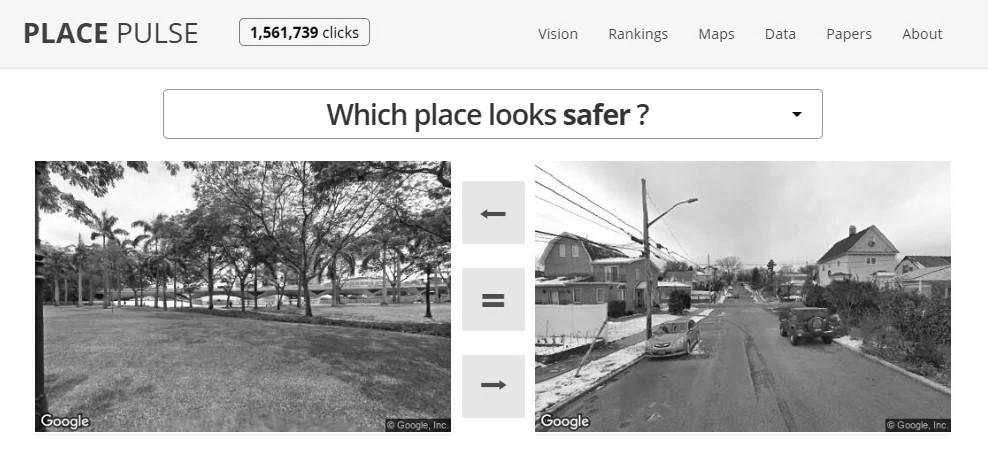
\includegraphics{figures/Place_Pulse.jpg}
\caption{Figure 1: Place Pulse website}
\end{figure}

\hypertarget{download-and-explore-place-pulse-data}{%
\subsection{3.2 Download and explore Place Pulse
data}\label{download-and-explore-place-pulse-data}}

We have saved some Place Pulse data in a data repository on FigShare.
You can download this directly into R by using the \texttt{read.csv()}
function. It is a large file so it may take some time to read in, be
patient!

\begin{Shaded}
\begin{Highlighting}[]
\NormalTok{pp_data <-}\StringTok{ }\KeywordTok{read.csv}\NormalTok{(}\StringTok{'https://ndownloader.figshare.com/files/21739137'}\NormalTok{) }
\end{Highlighting}
\end{Shaded}

This data set includes 17 variables, but we will only use some of them.
A unique identification code has been given to each participant (i.e.,
`voter\_uniqueid') and image, which can in the left (i.e.,
`place\_id\_left') or right (i.e., `place\_id\_right') part of each
pairwise comparison. The columns `place\_name\_left' and
`place\_name\_right' locate each image in its city. The column `choice'
shows if the user voted the image in the left, right, or equal, and the
column `study\_question' allows us to study perceptions about different
variables. `day' and `time' detail the moment when each vote toke place,
and the columns `long\_right', `lat\_right', `long\_left' and
`lat\_left' show the longitude and latitude of both images.

For instance, we can see which cities have a largest number of votes
amongst images in the left part of the pairwise comparison. To do this
we can use the \texttt{top\_n()} function from \texttt{dplyr} package:

CHANGE THIS TO TIDYVERSE -\textgreater{} group\_by \%\% summarise

\begin{Shaded}
\begin{Highlighting}[]
\NormalTok{pp_data }\OperatorTok
\StringTok{  }\KeywordTok{group_by}\NormalTok{(place_name_left) }\OperatorTok
\StringTok{  }\KeywordTok{summarize}\NormalTok{(}\DataTypeTok{Count =} \KeywordTok{n}\NormalTok{()) }\OperatorTok
\StringTok{  }\KeywordTok{top_n}\NormalTok{(}\DecValTok{5}\NormalTok{)}
\end{Highlighting}
\end{Shaded}

\begin{verbatim}
## # A tibble: 5 x 2
##   place_name_left Count
##   <fct>           <int>
## 1 Atlanta         56992
## 2 Berlin          55265
## 3 New York        48427
## 4 Rio De Janeiro  52725
## 5 Tokyo           53817
\end{verbatim}

Atlanta was the city with a largest number of votes. We can check if
that was also the case among pictures shown in the right part of the
comparison:

\begin{Shaded}
\begin{Highlighting}[]
\NormalTok{pp_data }\OperatorTok
\StringTok{  }\KeywordTok{group_by}\NormalTok{(place_name_right) }\OperatorTok
\StringTok{  }\KeywordTok{summarize}\NormalTok{(}\DataTypeTok{Count =} \KeywordTok{n}\NormalTok{()) }\OperatorTok
\StringTok{  }\KeywordTok{top_n}\NormalTok{(}\DecValTok{5}\NormalTok{)}
\end{Highlighting}
\end{Shaded}

\begin{verbatim}
## # A tibble: 5 x 2
##   place_name_right Count
##   <fct>            <int>
## 1 Atlanta          57140
## 2 Berlin           55583
## 3 Rio De Janeiro   52585
## 4 Santiago         48282
## 5 Tokyo            53514
\end{verbatim}

Atlanta was indeed the city with the largest number of votes. We can
also check which variables were more frequently assessed by
participants:

\begin{Shaded}
\begin{Highlighting}[]
\NormalTok{pp_data }\OperatorTok
\StringTok{  }\KeywordTok{group_by}\NormalTok{(study_question) }\OperatorTok
\StringTok{  }\KeywordTok{summarize}\NormalTok{(}\DataTypeTok{Count =} \KeywordTok{n}\NormalTok{())}
\end{Highlighting}
\end{Shaded}

\begin{verbatim}
## # A tibble: 7 x 2
##   study_question   Count
##   <fct>            <int>
## 1 livelier        366802
## 2 more beautiful  220604
## 3 more boring     144060
## 4 more depressing 149355
## 5 safer           509961
## 6 wealthier       174758
## 7 <NA>               183
\end{verbatim}

Safety was the most commonly assessed variable, with 509,961 votes in
total. Before analysing the data, we can also examine if participants
were more inclined to vote for images in the left or right part of the
platform.

\begin{Shaded}
\begin{Highlighting}[]
\NormalTok{pp_data }\OperatorTok
\StringTok{  }\KeywordTok{group_by}\NormalTok{(choice) }\OperatorTok
\StringTok{  }\KeywordTok{summarize}\NormalTok{(}\DataTypeTok{Count =} \KeywordTok{n}\NormalTok{()) }\OperatorTok
\StringTok{  }\KeywordTok{top_n}\NormalTok{(}\DecValTok{3}\NormalTok{)}
\end{Highlighting}
\end{Shaded}

\begin{verbatim}
## # A tibble: 3 x 2
##   choice  Count
##   <fct>   <int>
## 1 equal  206147
## 2 left   668680
## 3 right  690792
\end{verbatim}

The frequency of votes for left and right options is very similar, which
shows that the position of the image in the comparison does not have an
affect on participants' votes.

\hypertarget{cleaning-place-pulse-data}{%
\subsection{3.3 Cleaning Place Pulse
data}\label{cleaning-place-pulse-data}}

When it comes to crowdsourced data, you will have to be an expert data
wrangler to make sure you can get the data to behave like you want it to
- in other words to make the data available in a format that allows you
to answer your research questions. For example, in this case, we want to
map the perceives safety of areas in Atlanta. To do this, first we have
to select the area of Atlanta, and the votes about safety:

Let's focus on the city of Atlanta. SOME CONTEXT.

\begin{Shaded}
\begin{Highlighting}[]
\NormalTok{pp_atl <-}\StringTok{ }\NormalTok{pp_data[}\KeywordTok{which}\NormalTok{(pp_data}\OperatorTok{$}\NormalTok{place_name_right }\OperatorTok{==}\StringTok{ "Atlanta"} \OperatorTok{|}\StringTok{ }\NormalTok{pp_data}\OperatorTok{$}\NormalTok{place_name_left }\OperatorTok{==}\StringTok{ "Atlanta"}\NormalTok{), ]}
\end{Highlighting}
\end{Shaded}

Let's also focus on the ratings of areas as safer, as we are interested
in people's perceptions of the environment:

\begin{Shaded}
\begin{Highlighting}[]
\NormalTok{pp_atl_s <-}\StringTok{ }\NormalTok{pp_atl[ }\KeywordTok{which}\NormalTok{(pp_atl}\OperatorTok{$}\NormalTok{study_question }\OperatorTok{==}\StringTok{ "safer"}\NormalTok{), ]}
\end{Highlighting}
\end{Shaded}

You can see now we have a dataframe of 37214 votes about the safety of
places in Atlanta.

We are interested in analysing the proportion of `safer' votes in each
neighbourhood of Atlanta. We will create two new columns that specify
the longitude and latitude of the image of Atlanta being assessed by
participant, and we will also create one new column that details whether
the user votes that the image of Atlanta was `safer' or not safer than
another picture. Some pairwise comparisons, nevetheless, assessed two
images from Atlanta, which means that we will need to duplicate these
votes to account for both the image assessed as `safer' and the picture
reported as `not safer'. First, we want to know the number of
comparisons in which both images are from Atlanta.

\begin{Shaded}
\begin{Highlighting}[]
\KeywordTok{table}\NormalTok{(pp_atl_s}\OperatorTok{$}\NormalTok{place_name_right }\OperatorTok{==}\StringTok{ "Atlanta"} \OperatorTok{&}\StringTok{ }\NormalTok{pp_atl_s}\OperatorTok{$}\NormalTok{place_name_left }\OperatorTok{==}\StringTok{ "Atlanta"}\NormalTok{) }\CommentTok{#count votes in which both images are from Atlanta}
\end{Highlighting}
\end{Shaded}

\begin{verbatim}
## 
## FALSE  TRUE 
## 36536   678
\end{verbatim}

In total, 678 pairwise comparisons included in our dataset are based on
two images from the city of Atlanta, whereas 36,536 compare one image
from Atlanta with a picture from another city. We will duplicate those
comparisons in which both images were taken in Atlanta and attach them
to two new datasets (one to assess the images on the right, and the
other to report the images on the left). For now, we delete these cases
from the main dataframe, but we will merge them once all the data has
been cleaned.

\begin{Shaded}
\begin{Highlighting}[]
\NormalTok{pp_atl_s <-}\StringTok{ }\NormalTok{pp_atl_s[}\KeywordTok{order}\NormalTok{(pp_atl_s}\OperatorTok{$}\NormalTok{X), ] }\CommentTok{#order file by vote number}

\NormalTok{pp_atl_s_dup <-}\StringTok{ }\NormalTok{pp_atl_s[}\KeywordTok{which}\NormalTok{(pp_atl_s}\OperatorTok{$}\NormalTok{place_name_right }\OperatorTok{==}\StringTok{ "Atlanta"} \OperatorTok{&}\StringTok{ }\NormalTok{pp_atl_s}\OperatorTok{$}\NormalTok{place_name_left }\OperatorTok{==}\StringTok{ "Atlanta"}\NormalTok{), ] }\CommentTok{#new dataset: both images are from Atlanta}
\NormalTok{pp_atl_s_dup2 <-}\StringTok{ }\NormalTok{pp_atl_s_dup }\CommentTok{#duplicate new dataset}

\NormalTok{pp_atl_s <-}\StringTok{ }\NormalTok{pp_atl_s[}\OperatorTok{!}\NormalTok{(pp_atl_s}\OperatorTok{$}\NormalTok{X }\OperatorTok\StringTok{ }\NormalTok{pp_atl_s_dup}\OperatorTok{$}\NormalTok{X), ] }\CommentTok{#delete duplicated votes from main dataset}
\end{Highlighting}
\end{Shaded}

Now, the main dataset only includes those pairwise comparison in which
only one image was from Atlanta. We create two new columns that specify
the coordinates of the picture from Atlanta in which we are interested.
First, we allocate the coordinates to those votes in which the image of
the left is from Atlanta:

\begin{Shaded}
\begin{Highlighting}[]
\NormalTok{pp_atl_s}\OperatorTok{$}\NormalTok{long_Atl[pp_atl_s}\OperatorTok{$}\NormalTok{place_name_left }\OperatorTok{==}\StringTok{ "Atlanta"}\NormalTok{] <-}\StringTok{ }\NormalTok{pp_atl_s}\OperatorTok{$}\NormalTok{long_left[pp_atl_s}\OperatorTok{$}\NormalTok{place_name_left }\OperatorTok{==}\StringTok{ "Atlanta"}\NormalTok{]}
\NormalTok{pp_atl_s}\OperatorTok{$}\NormalTok{lat_Atl[pp_atl_s}\OperatorTok{$}\NormalTok{place_name_left }\OperatorTok{==}\StringTok{ "Atlanta"}\NormalTok{] <-}\StringTok{ }\NormalTok{pp_atl_s}\OperatorTok{$}\NormalTok{lat_left[pp_atl_s}\OperatorTok{$}\NormalTok{place_name_left }\OperatorTok{==}\StringTok{ "Atlanta"}\NormalTok{]}
\end{Highlighting}
\end{Shaded}

We then reproduce the same step with those votes in which the right
image is from Atlanta:

\begin{Shaded}
\begin{Highlighting}[]
\NormalTok{pp_atl_s}\OperatorTok{$}\NormalTok{long_Atl[pp_atl_s}\OperatorTok{$}\NormalTok{place_name_right }\OperatorTok{==}\StringTok{ "Atlanta"}\NormalTok{] <-}\StringTok{ }\NormalTok{pp_atl_s}\OperatorTok{$}\NormalTok{long_right[pp_atl_s}\OperatorTok{$}\NormalTok{place_name_right }\OperatorTok{==}\StringTok{ "Atlanta"}\NormalTok{] }
\NormalTok{pp_atl_s}\OperatorTok{$}\NormalTok{lat_Atl[pp_atl_s}\OperatorTok{$}\NormalTok{place_name_right }\OperatorTok{==}\StringTok{ "Atlanta"}\NormalTok{] <-}\StringTok{ }\NormalTok{pp_atl_s}\OperatorTok{$}\NormalTok{lat_right[pp_atl_s}\OperatorTok{$}\NormalTok{place_name_right }\OperatorTok{==}\StringTok{ "Atlanta"}\NormalTok{]}
\end{Highlighting}
\end{Shaded}

Remember that we had previously created two new datasets with those
votes in which both images are from Atlanta. The first dataset
(`pp\_atl\_s\_dup') will be used to assess the images in the left, while
the second dataset (`pp\_atl\_s\_dup2') will refer to the images in the
right. We can then allocate the coordinates of the left image to first
dataset of votes in which both images are from Atlanta:

\begin{Shaded}
\begin{Highlighting}[]
\NormalTok{pp_atl_s_dup}\OperatorTok{$}\NormalTok{long_Atl <-}\StringTok{ }\NormalTok{pp_atl_s_dup}\OperatorTok{$}\NormalTok{long_left}
\NormalTok{pp_atl_s_dup}\OperatorTok{$}\NormalTok{lat_Atl <-}\StringTok{ }\NormalTok{pp_atl_s_dup}\OperatorTok{$}\NormalTok{lat_left}
\end{Highlighting}
\end{Shaded}

And then allocate the coordinates of the right image to the second
dataset of pairwise comparisons between Atlanta pictures:

\begin{Shaded}
\begin{Highlighting}[]
\NormalTok{pp_atl_s_dup2}\OperatorTok{$}\NormalTok{long_Atl <-}\StringTok{ }\NormalTok{pp_atl_s_dup2}\OperatorTok{$}\NormalTok{long_right}
\NormalTok{pp_atl_s_dup2}\OperatorTok{$}\NormalTok{lat_Atl <-}\StringTok{ }\NormalTok{pp_atl_s_dup2}\OperatorTok{$}\NormalTok{lat_right}
\end{Highlighting}
\end{Shaded}

Before merging all the data into a single dataset, we will create a new
column that distinguished those images of Atlanta that were assessed as
`safer' from those reported as "less safe' or `equal'. We can do this
first in the main dataset (which only includes pairwise comparisons with
one picture from Atlanta), by checking if the option of each user (i.e.,
`left', `right', or `equal') correspond to the city of the image of
Atlanta. We assign a 1 when the users' vote corresponds to the position
of the image of Atlanta, whereas a 0 is assigned when the image of a
different city was chosen to be `safer' and when users voted `equal'.

\begin{Shaded}
\begin{Highlighting}[]
\NormalTok{pp_atl_s}\OperatorTok{$}\NormalTok{win[pp_atl_s}\OperatorTok{$}\NormalTok{place_name_left }\OperatorTok{==}\StringTok{ "Atlanta"} \OperatorTok{&}\StringTok{ }\NormalTok{pp_atl_s}\OperatorTok{$}\NormalTok{choice }\OperatorTok{==}\StringTok{ "left"}\NormalTok{] <-}\StringTok{ }\DecValTok{1}
\NormalTok{pp_atl_s}\OperatorTok{$}\NormalTok{win[pp_atl_s}\OperatorTok{$}\NormalTok{place_name_left }\OperatorTok{==}\StringTok{ "Atlanta"} \OperatorTok{&}\StringTok{ }\NormalTok{pp_atl_s}\OperatorTok{$}\NormalTok{choice }\OperatorTok{==}\StringTok{ "right"}\NormalTok{] <-}\StringTok{ }\DecValTok{0}
\NormalTok{pp_atl_s}\OperatorTok{$}\NormalTok{win[pp_atl_s}\OperatorTok{$}\NormalTok{place_name_left }\OperatorTok{==}\StringTok{ "Atlanta"} \OperatorTok{&}\StringTok{ }\NormalTok{pp_atl_s}\OperatorTok{$}\NormalTok{choice }\OperatorTok{==}\StringTok{ "equal"}\NormalTok{] <-}\StringTok{ }\DecValTok{0}

\NormalTok{pp_atl_s}\OperatorTok{$}\NormalTok{win[pp_atl_s}\OperatorTok{$}\NormalTok{place_name_right }\OperatorTok{==}\StringTok{ "Atlanta"} \OperatorTok{&}\StringTok{ }\NormalTok{pp_atl_s}\OperatorTok{$}\NormalTok{choice }\OperatorTok{==}\StringTok{ "right"}\NormalTok{] <-}\StringTok{ }\DecValTok{1}
\NormalTok{pp_atl_s}\OperatorTok{$}\NormalTok{win[pp_atl_s}\OperatorTok{$}\NormalTok{place_name_right }\OperatorTok{==}\StringTok{ "Atlanta"} \OperatorTok{&}\StringTok{ }\NormalTok{pp_atl_s}\OperatorTok{$}\NormalTok{choice }\OperatorTok{==}\StringTok{ "left"}\NormalTok{] <-}\StringTok{ }\DecValTok{0}
\NormalTok{pp_atl_s}\OperatorTok{$}\NormalTok{win[pp_atl_s}\OperatorTok{$}\NormalTok{place_name_right }\OperatorTok{==}\StringTok{ "Atlanta"} \OperatorTok{&}\StringTok{ }\NormalTok{pp_atl_s}\OperatorTok{$}\NormalTok{choice }\OperatorTok{==}\StringTok{ "equal"}\NormalTok{] <-}\StringTok{ }\DecValTok{0}
\end{Highlighting}
\end{Shaded}

Similarly, we can assign a 1 to the `pp\_atl\_s\_dup' when the users
voted that the left image looked `safer' and a 0 otherwise, given that
this dataset has been previously created to assess the images of the
left of pairwise comparisons in which both images were from Atlanta. And
we can do the same with the second dataset that compares two images from
Atlanta, which in this case refers to the image in the right.

\begin{Shaded}
\begin{Highlighting}[]
\NormalTok{pp_atl_s_dup}\OperatorTok{$}\NormalTok{win[pp_atl_s_dup}\OperatorTok{$}\NormalTok{choice }\OperatorTok{==}\StringTok{ "left"}\NormalTok{] <-}\StringTok{ }\DecValTok{1}
\NormalTok{pp_atl_s_dup}\OperatorTok{$}\NormalTok{win[pp_atl_s_dup}\OperatorTok{$}\NormalTok{choice }\OperatorTok{==}\StringTok{ "right"}\NormalTok{] <-}\StringTok{ }\DecValTok{0}
\NormalTok{pp_atl_s_dup}\OperatorTok{$}\NormalTok{win[pp_atl_s_dup}\OperatorTok{$}\NormalTok{choice }\OperatorTok{==}\StringTok{ "equal"}\NormalTok{] <-}\StringTok{ }\DecValTok{0}

\NormalTok{pp_atl_s_dup2}\OperatorTok{$}\NormalTok{win[pp_atl_s_dup}\OperatorTok{$}\NormalTok{choice }\OperatorTok{==}\StringTok{ "right"}\NormalTok{] <-}\StringTok{ }\DecValTok{1}
\NormalTok{pp_atl_s_dup2}\OperatorTok{$}\NormalTok{win[pp_atl_s_dup}\OperatorTok{$}\NormalTok{choice }\OperatorTok{==}\StringTok{ "left"}\NormalTok{] <-}\StringTok{ }\DecValTok{0}
\NormalTok{pp_atl_s_dup2}\OperatorTok{$}\NormalTok{win[pp_atl_s_dup}\OperatorTok{$}\NormalTok{choice }\OperatorTok{==}\StringTok{ "equal"}\NormalTok{] <-}\StringTok{ }\DecValTok{0}
\end{Highlighting}
\end{Shaded}

Now that our dataset has been cleaned and is ready to be analysed, we
can merge all the data together.

\begin{Shaded}
\begin{Highlighting}[]
\NormalTok{pp_atl_s <-}\StringTok{ }\KeywordTok{rbind}\NormalTok{(pp_atl_s, pp_atl_s_dup, pp_atl_s_dup2) }
\end{Highlighting}
\end{Shaded}

table(pp\_atl\_s\(win) #count frequency of 'safer' votes in Atlanta against 'equal' and 'less safe' votes prop.table(table(pp_atl_s\)win))*100
\#count \% of `safer' votes in Atlanta against `equal' and `less safe'
votes

\begin{verbatim}

## 3.4 Map Place Pulse data

It is possible to use mapping techniques learned in other chapters (LINK WITH MAPPING CHAPTER PEOPLE) to map the crowdsourced data. 

 Let's plot this, to create a map of perceived safety of built environment across the city of Atlanta. For this, we will be using the `sf` and `ggplot2` libraries. 

First, acquire a shapefile for Atlanta. Let's use the neighbourhoods shapefile from the department of city planning. You can go on their website to find out more about this boundary data: [https://dcp-coaplangis.opendata.arcgis.com/datasets/neighborhoods](https://dcp-coaplangis.opendata.arcgis.com/datasets/neighborhoods). We can download the shapefile directly using their Application Programme Interfact (or API) - this is something discussed in greater detail on the chapter on Open Data (CHAPTER REF). For now, you can just use the code below, with the `st_read()` function in the `sf` package: 


```r
#atl <- st_read("https://opendata.arcgis.com/datasets/297d3d69d8ab4c6ba5f9264ad5e75c0a_3.geojson")

atl <- st_read("http://worldmap.harvard.edu/download/wfs/1824/json?outputFormat=json&service=WFS&request=GetFeature&format_options=charset%3AUTF-8&typename=geonode%3AAtlanta_Census_Tracts_SHL&version=1.0.0")
\end{verbatim}

\begin{verbatim}
## Reading layer `OGRGeoJSON' from data source `http://worldmap.harvard.edu/download/wfs/1824/json?outputFormat=json&service=WFS&request=GetFeature&format_options=charset%3AUTF-8&typename=geonode%3AAtlanta_Census_Tracts_SHL&version=1.0.0' using driver `GeoJSON'
## Simple feature collection with 799 features and 29 fields
## geometry type:  MULTIPOLYGON
## dimension:      XY
## bbox:           xmin: -85.65203 ymin: 32.96982 xmax: -82.94681 ymax: 34.58748
## epsg (SRID):    4326
## proj4string:    +proj=longlat +datum=WGS84 +no_defs
\end{verbatim}

We can see what this looks like by using the \texttt{plot()} function to
plot the geometry of the atl object we created, called with the
\texttt{st\_geometry()} function:

\begin{Shaded}
\begin{Highlighting}[]
\KeywordTok{plot}\NormalTok{(}\KeywordTok{st_geometry}\NormalTok{(atl))}
\end{Highlighting}
\end{Shaded}

\includegraphics{chapter_files/figure-latex/plotatlgeom-1.pdf}

Now to be able to plot the safety votes on this map, we first need to
make our votes a spatial object, by specfying that the ``long\_Atl'' and
``lat\_Atl'' contain our longitude and latitude information. We use the
\texttt{st\_as\_sf()} function for this:

\begin{Shaded}
\begin{Highlighting}[]
\NormalTok{points_atl_s <-}\StringTok{ }\KeywordTok{st_as_sf}\NormalTok{(pp_atl_s, }\DataTypeTok{coords =} \KeywordTok{c}\NormalTok{(}\StringTok{"lat_Atl"}\NormalTok{, }\StringTok{"long_Atl"}\NormalTok{)) }\CommentTok{#geocode 'safe' votes in Atlanta}
\end{Highlighting}
\end{Shaded}

Now to be able to plot both these spatial layers on the same map, their
coordinate reference systems need to match. We can check these with the
\texttt{st\_crs()} function:

\begin{Shaded}
\begin{Highlighting}[]
\KeywordTok{st_crs}\NormalTok{(points_atl_s) }\OperatorTok{==}\StringTok{ }\KeywordTok{st_crs}\NormalTok{(atl) }\CommentTok{#check if coordinate reference system is the same of both layers}
\end{Highlighting}
\end{Shaded}

\begin{verbatim}
## [1] FALSE
\end{verbatim}

\begin{Shaded}
\begin{Highlighting}[]
\KeywordTok{st_crs}\NormalTok{(points_atl_s) <-}\StringTok{ }\KeywordTok{st_crs}\NormalTok{(atl)}
\end{Highlighting}
\end{Shaded}

Now if we check, they should have the same CRS:

\begin{Shaded}
\begin{Highlighting}[]
\KeywordTok{st_crs}\NormalTok{(points_atl_s) }\OperatorTok{==}\StringTok{ }\KeywordTok{st_crs}\NormalTok{(atl) }\CommentTok{#check if coordinate reference system is the same of both layers}
\end{Highlighting}
\end{Shaded}

\begin{verbatim}
## [1] TRUE
\end{verbatim}

Indeed! Now we can map our data!

\begin{Shaded}
\begin{Highlighting}[]
\NormalTok{map <-}\StringTok{ }\KeywordTok{ggplot}\NormalTok{(}\DataTypeTok{data =}\NormalTok{ atl) }\OperatorTok{+}\StringTok{ }\KeywordTok{geom_sf}\NormalTok{() }\OperatorTok{+}\StringTok{ }\KeywordTok{theme_void}\NormalTok{() }\OperatorTok{+}
\StringTok{  }\KeywordTok{coord_sf}\NormalTok{(}\DataTypeTok{xlim =} \KeywordTok{c}\NormalTok{(}\OperatorTok{-}\DecValTok{84}\NormalTok{, }\FloatTok{-84.7}\NormalTok{), }\DataTypeTok{ylim =} \KeywordTok{c}\NormalTok{(}\FloatTok{33.6}\NormalTok{, }\DecValTok{34}\NormalTok{), }\DataTypeTok{expand =} \OtherTok{FALSE}\NormalTok{) }\CommentTok{#create map}
  
\NormalTok{map }\OperatorTok{+}\StringTok{ }\KeywordTok{geom_point}\NormalTok{(}\DataTypeTok{data =}\NormalTok{ pp_atl_s, }\KeywordTok{aes}\NormalTok{(}\DataTypeTok{x =}\NormalTok{ lat_Atl, }\DataTypeTok{y =}\NormalTok{ long_Atl), }\DataTypeTok{size =} \FloatTok{.1}\NormalTok{) }\CommentTok{#plot map with points}
\end{Highlighting}
\end{Shaded}

\includegraphics{chapter_files/figure-latex/plotpoints-1.pdf}

This is a very busy map! Maybe instead we want to get some sort of
average score for each neighbourhood.

Get win score for each nhood

\begin{Shaded}
\begin{Highlighting}[]
\NormalTok{points_atl_s_nhood <-}\StringTok{ }\KeywordTok{st_intersection}\NormalTok{(atl, points_atl_s) }\OperatorTok\StringTok{ }
\StringTok{  }\KeywordTok{group_by}\NormalTok{(TRACT) }\OperatorTok\StringTok{ }
\StringTok{  }\KeywordTok{summarise}\NormalTok{(}\DataTypeTok{winscore =} \KeywordTok{mean}\NormalTok{(win, }\DataTypeTok{na.rm =} \OtherTok{TRUE}\NormalTok{), }
            \DataTypeTok{num_votes =} \KeywordTok{n}\NormalTok{())}
\end{Highlighting}
\end{Shaded}

Join to shapefile and delete areas with zero votes

\begin{Shaded}
\begin{Highlighting}[]
\KeywordTok{st_geometry}\NormalTok{(points_atl_s_nhood) <-}\StringTok{ }\OtherTok{NULL}

\NormalTok{atl_pp_wins <-}\StringTok{ }\KeywordTok{left_join}\NormalTok{(atl, points_atl_s_nhood, }\DataTypeTok{by =} \KeywordTok{c}\NormalTok{(}\StringTok{"TRACT"}\NormalTok{ =}\StringTok{ "TRACT"}\NormalTok{))}

\NormalTok{atl_pp_wins <-}\StringTok{ }\NormalTok{atl_pp_wins[}\OperatorTok{!}\KeywordTok{is.na}\NormalTok{(atl_pp_wins}\OperatorTok{$}\NormalTok{winscore), ]}
\end{Highlighting}
\end{Shaded}

\begin{Shaded}
\begin{Highlighting}[]
\KeywordTok{ggplot}\NormalTok{(}\DataTypeTok{data =}\NormalTok{ atl_pp_wins) }\OperatorTok{+}\StringTok{ }
\StringTok{  }\KeywordTok{geom_sf}\NormalTok{(}\KeywordTok{aes}\NormalTok{(}\DataTypeTok{fill =}\NormalTok{ winscore)) }\OperatorTok{+}
\StringTok{  }\KeywordTok{coord_sf}\NormalTok{(}\DataTypeTok{xlim =} \KeywordTok{c}\NormalTok{(}\OperatorTok{-}\DecValTok{84}\NormalTok{, }\FloatTok{-84.7}\NormalTok{), }\DataTypeTok{ylim =} \KeywordTok{c}\NormalTok{(}\FloatTok{33.5}\NormalTok{, }\DecValTok{34}\NormalTok{), }\DataTypeTok{expand =} \OtherTok{FALSE}\NormalTok{) }\OperatorTok{+}
\StringTok{  }\KeywordTok{theme_void}\NormalTok{() }
\end{Highlighting}
\end{Shaded}

\includegraphics{chapter_files/figure-latex/mapwins-1.pdf}

About this: Note: @salesses2013 suggest computing a Q-score corrected by
the ``win'' and ``loss'' ratio of imagines with which each vote is
compared for the purpose of this chapter we will compute a simple
proportion - should we include this for an activity?

There are many more things you can do with these data. for example you
could look at the descriptive statistics:

\begin{Shaded}
\begin{Highlighting}[]
\KeywordTok{summary}\NormalTok{(atl_pp_wins}\OperatorTok{$}\NormalTok{winscore) }\CommentTok{#descriptive statistics of proportion of 'safer' votes per tract}
\end{Highlighting}
\end{Shaded}

\begin{verbatim}
##    Min. 1st Qu.  Median    Mean 3rd Qu.    Max. 
##  0.1111  0.4256  0.4907  0.4784  0.5362  0.6842
\end{verbatim}

Important also to consider variation in the sample size of number of
votes in each neighbourhood:

\begin{Shaded}
\begin{Highlighting}[]
\KeywordTok{summary}\NormalTok{(atl_pp_wins}\OperatorTok{$}\NormalTok{num_votes)}
\end{Highlighting}
\end{Shaded}

\begin{verbatim}
##    Min. 1st Qu.  Median    Mean 3rd Qu.    Max. 
##    2.00   80.25  138.50  183.39  242.00 1048.00
\end{verbatim}

Talk a little about the issues with this and then discuss this: Note:
Buil-Gil et al.~(2020) propose a new method to compute estimates for
areas with small sample sizes

You can do much more, but here we will focus on the specific issues to
explore due to the crowdsourced nature of these data!

\hypertarget{exploring-the-known-issues-of-crowdsourced-data-within-place-pulse}{%
\subsection{3.5 Exploring the known issues of crowdsourced data within
Place
Pulse}\label{exploring-the-known-issues-of-crowdsourced-data-within-place-pulse}}

We mentioned a few issues that are usually present in crowdsourced data,
and which are important to keep in mind. Here we explore whether they
are present in Place Pulse, and what that might mean for any conclusions
we draw from our analyses.

First, create a new dataframe showing the number of votes that each
study participant had made. To do this, we will use code from the
\texttt{dplyr} library:

\begin{Shaded}
\begin{Highlighting}[]
\NormalTok{voter <-}\StringTok{ }\NormalTok{pp_data }\OperatorTok\StringTok{ }
\StringTok{  }\KeywordTok{group_by}\NormalTok{(voter_uniqueid) }\OperatorTok\StringTok{ }
\StringTok{  }\KeywordTok{summarise}\NormalTok{(}\DataTypeTok{num_votes =} \KeywordTok{n}\NormalTok{())}
\end{Highlighting}
\end{Shaded}

If you want, you can have a look at this new dataframe using the
\texttt{View()} function. If you do this, you might see, we have some
very active participants! The top voter there has made 7168 votes on
places! That is some very prolific participation! On the other hand, you
can also see that 7494 of the participants made only one vote! We are
definitely seeing signs of participation inequality in these data.

\hypertarget{participation-inequality-supercontributors}{%
\subsubsection{3.5.1 Participation inequality
(supercontributors)}\label{participation-inequality-supercontributors}}

In fact, let's see, how much of the votes do the ``supercontributors''
account for? Let's say we want to consider the top 1\% of voters. We can
do this using the \texttt{subset()} and \texttt{quantile()} functions:

\begin{Shaded}
\begin{Highlighting}[]
\NormalTok{top_1percent <-}\StringTok{ }\KeywordTok{subset}\NormalTok{(voter, num_votes }\OperatorTok{>}\StringTok{ }\KeywordTok{quantile}\NormalTok{(num_votes, }\DataTypeTok{prob =} \DecValTok{1} \OperatorTok{-}\StringTok{ }\DecValTok{1}\OperatorTok{/}\DecValTok{100}\NormalTok{)) }
\end{Highlighting}
\end{Shaded}

We can see that this new dataframe contains 954 people, who are our top
1\% contributors to the Place Plus data set. Let's see how much of the
total number of votes they contribute:

\begin{Shaded}
\begin{Highlighting}[]
\KeywordTok{sum}\NormalTok{(top_1percent}\OperatorTok{$}\NormalTok{num_votes) }\OperatorTok{/}\StringTok{ }\KeywordTok{sum}\NormalTok{(voter}\OperatorTok{$}\NormalTok{num_votes) }\OperatorTok{*}\StringTok{ }\DecValTok{100}
\end{Highlighting}
\end{Shaded}

\begin{verbatim}
## [1] 17.87468
\end{verbatim}

That is a lot! 17.87\% of the votes are made by the top 1\% of
contributors!

\hypertarget{activity-1}{%
\paragraph{Activity 1}\label{activity-1}}

Can you tell me what proportion of the votes were made by the top 10\%
of participants? What about the top 25\%?

\hypertarget{quantifying-participation-inequality}{%
\subsubsection{3.5.2 Quantifying participation
inequality}\label{quantifying-participation-inequality}}

One way to quantify the extent to which participation inequality exists
in our data is by using a Gini index, and visualising using a Lorenz
curve.

For this you will need the library \texttt{ineq} so if you don't already
have this you must install with the command:

\begin{Shaded}
\begin{Highlighting}[]
\KeywordTok{install.packages}\NormalTok{(}\StringTok{"ineq"}\NormalTok{) }
\end{Highlighting}
\end{Shaded}

Then you can load this library and calculate the index using the
\texttt{Gini()} function:

\begin{Shaded}
\begin{Highlighting}[]
\KeywordTok{Gini}\NormalTok{(voter}\OperatorTok{$}\NormalTok{num_votes)}
\end{Highlighting}
\end{Shaded}

\begin{verbatim}
## [1] 0.5777568
\end{verbatim}

Remember that a score of 0 is perfect equality (everyone makes equal
number of votes), while 1 is perfect inequality (only one person making
all the reports, and no one else making any) . Our answer of 0.58 shows
some serious inequality. To put this into context, in 2017, according to
the OECD, income inequality in the United States of America showed a
Gini coefficient of 0.39.\\
To visualise this we can use a Lorenz curve using the \texttt{plot()}
and \texttt{Lc()} functions:

\begin{Shaded}
\begin{Highlighting}[]
\KeywordTok{plot}\NormalTok{(}\KeywordTok{Lc}\NormalTok{(voter}\OperatorTok{$}\NormalTok{num_votes), }\DataTypeTok{xlab =} \StringTok{"Cumulative share of participants from lowest to higher number of votes"}\NormalTok{,}
     \DataTypeTok{ylab =} \StringTok{"Cumulative share of votes"}\NormalTok{,}\DataTypeTok{col=}\StringTok{"darkred"}\NormalTok{,}\DataTypeTok{lwd=}\DecValTok{2}\NormalTok{) }
\end{Highlighting}
\end{Shaded}

\includegraphics{chapter_files/figure-latex/lorenz-1.pdf}

The Lorenz curve (red line) above shows how the top few percent of
reporters contribute the majority of the reports. If we had perfect
equality, we would expect to see the red line align perfectly with the
black line with the slope of 1.

With this information we can now quantify how severe the participation
inequality in our data, and compare with other crowdsourced data for
context and understanding.

\hypertarget{study-participation-descrease-in-place-pulse}{%
\subsubsection{3.5.3 Study participation descrease in Place
Pulse}\label{study-participation-descrease-in-place-pulse}}

!!!This should also be broken up and motivated/exaplained!!!

\begin{Shaded}
\begin{Highlighting}[]
\NormalTok{by_day <-}\StringTok{ }\NormalTok{pp_data }\OperatorTok\StringTok{ }
\StringTok{  }\KeywordTok{mutate}\NormalTok{(}\DataTypeTok{day =} \KeywordTok{ymd}\NormalTok{(day)) }\OperatorTok\StringTok{ }
\StringTok{  }\KeywordTok{group_by}\NormalTok{(day) }\OperatorTok\StringTok{ }
\StringTok{  }\KeywordTok{summarise}\NormalTok{(}\DataTypeTok{num_votes =} \KeywordTok{n}\NormalTok{()) }\OperatorTok\StringTok{ }
\StringTok{  }\KeywordTok{complete}\NormalTok{(}\DataTypeTok{day =} \KeywordTok{seq.Date}\NormalTok{(}\KeywordTok{min}\NormalTok{(day), }\KeywordTok{max}\NormalTok{(day), }\DataTypeTok{by=}\StringTok{"day"}\NormalTok{)) }\OperatorTok\StringTok{ }
\StringTok{  }\KeywordTok{mutate}\NormalTok{(}\DataTypeTok{num_votes =} \KeywordTok{replace_na}\NormalTok{(num_votes, }\DecValTok{0}\NormalTok{))}


\KeywordTok{ggplot}\NormalTok{(by_day, }\KeywordTok{aes}\NormalTok{(}\DataTypeTok{x =}\NormalTok{ day, }\DataTypeTok{y =}\NormalTok{ num_votes)) }\OperatorTok{+}\StringTok{ }
\StringTok{  }\KeywordTok{geom_line}\NormalTok{() }\OperatorTok{+}\StringTok{ }
\StringTok{  }\KeywordTok{geom_smooth}\NormalTok{(}\DataTypeTok{lwd =} \FloatTok{1.5}\NormalTok{, }\DataTypeTok{col =} \StringTok{"red"}\NormalTok{) }\OperatorTok{+}\StringTok{ }
\StringTok{  }\KeywordTok{theme_bw}\NormalTok{() }\OperatorTok{+}\StringTok{ }
\StringTok{  }\KeywordTok{xlab}\NormalTok{(}\StringTok{"Days since website launch"}\NormalTok{) }\OperatorTok{+}\StringTok{ }
\StringTok{  }\KeywordTok{ylab}\NormalTok{(}\StringTok{"Number of votes"}\NormalTok{) }
\end{Highlighting}
\end{Shaded}

\includegraphics{chapter_files/figure-latex/datestuff-1.pdf}

Note: large peak beginning on July 24th 2013: publication of
@salesses2013 on July 24th and press release via MIT News
(\url{http://news.mit.edu/2013/quantifying-urban-perceptions-0724})
Note: large peak beginning on October 15th 2014: publication of
@Harvey2014 MSc thesis

\hypertarget{measure-validity}{%
\subsubsection{3.4.4 Measure validity}\label{measure-validity}}

Validity of an assessment is the degree to which it measures what it is
supposed to measure.

\hypertarget{wrap-upwhere-to-next}{%
\section{Wrap-up/Where to next:}\label{wrap-upwhere-to-next}}

\hypertarget{open-topics-in-crowdsourced-data}{%
\subsection{Open topics in crowdsourced
data}\label{open-topics-in-crowdsourced-data}}

\hypertarget{further-applications-to-crime-and-place-research}{%
\subsection{Further applications to crime and place
research}\label{further-applications-to-crime-and-place-research}}

\end{document}
